%%%%%%%%%%%%%%%%%%%%%%%%%%%%%%%%%%%%%%%%%%%%%%%%%%%%%%%%%%%%%%%%%%%%%%
% LaTeX Template: Curriculum Vitae
%
% Source: http://www.howtotex.com/
% Feel free to distribute this template, but please keep the
% referal to HowToTeX.com.
% Date: July 2011
% 
%%%%%%%%%%%%%%%%%%%%%%%%%%%%%%%%%%%%%%%%%%%%%%%%%%%%%%%%%%%%%%%%%%%%%%
% How to use writeLaTeX: 
%
% You edit the source code here on the left, and the preview on the
% right shows you the result within a few seconds.
%
% Bookmark this page and share the URL with your co-authors. They can
% edit at the same time!
%
% You can upload figures, bibliographies, custom classes and
% styles using the files menu.
%
% If you're new to LaTeX, the wikibook is a great place to start:
% http://en.wikibooks.org/wiki/LaTeX
%
%%%%%%%%%%%%%%%%%%%%%%%%%%%%%%%%%%%%%%%%%%%%%%%%%%%%%%%%%%%%%%%%%%%%%%
\documentclass[paper=a4,fontsize=11pt]{scrartcl} % KOMA-article class
							
\usepackage[english]{babel}
\usepackage[utf8x]{inputenc}
\usepackage[protrusion=true,expansion=true]{microtype}
\usepackage{amsmath,amsfonts,amsthm}     % Math packages
\usepackage{graphicx}                    % Enable pdflatex
\usepackage{wrapfig}
\usepackage[svgnames]{xcolor}            % Colors by their 'svgnames'
\usepackage{geometry}
	\textheight=700px                    % Saving trees ;-)
\usepackage{url}

\frenchspacing              % Better looking spacings after periods
\pagestyle{empty}           % No pagenumbers/headers/footers

%%% Custom sectioning (sectsty package)
%%% ------------------------------------------------------------
\usepackage{sectsty}

\sectionfont{%			            % Change font of \section command
	\usefont{OT1}{phv}{b}{n}%		% bch-b-n: CharterBT-Bold font
	\sectionrule{0pt}{0pt}{-5pt}{3pt}}

%%% Macros
%%% ------------------------------------------------------------
\newlength{\spacebox}
\settowidth{\spacebox}{8888888888}			% Box to align text
\newcommand{\sepspace}{\vspace*{1em}}		% Vertical space macro

\newcommand{\MyName}[1]{ % Name
		\Huge \usefont{OT1}{phv}{b}{n} \hfill #1
		\par \normalsize \normalfont}
		
\newcommand{\MySlogan}[1]{ % Slogan (optional)
		\large \usefont{OT1}{phv}{m}{n}\hfill \textit{#1}
		\par \normalsize \normalfont}

\newcommand{\NewPart}[1]{\section*{\uppercase{#1}}}

\newcommand{\PersonalEntry}[2]{
		\noindent\hangindent=2em\hangafter=0 % Indentation
		\parbox{\spacebox}{        % Box to align text
		\textit{#1}}		       % Entry name (birth, address, etc.)
		\hspace{1.5em} #2 \par}    % Entry value

\newcommand{\ObjectivesEntry}[2]{      % Same as \PersonalEntry
		\noindent\hangindent=2em\hangafter=0 % Indentation
		\parbox{\spacebox}{        % Box to align text
		\textit{#1}}			   % Entry name (birth, address, etc.)
		\hspace{1.5em} #2 \par}    % Entry value	

\newcommand{\SkillsEntry}[2]{      % Same as \PersonalEntry
		\noindent\hangindent=2em\hangafter=0 % Indentation
		\parbox{\spacebox}{        % Box to align text
		\textit{#1}}			   % Entry name (birth, address, etc.)
		\hspace{1.5em} #2 \par}    % Entry value	
		
\newcommand{\EducationEntry}[4]{
		\noindent \textbf{#1} \hfill      % Study
		\colorbox{Black}{%
			\parbox{6em}{%
			\hfill\color{White}#2}} \par  % Duration
		\noindent \textit{#3} \par        % School
		\noindent\hangindent=2em\hangafter=0 \small #4 % Description
		\normalsize \par}

\newcommand{\WorkEntry}[4]{				  % Same as \EducationEntry
		\noindent \textbf{#1} \hfill      % Jobname
		\colorbox{Black}{\color{White}#2} \par  % Duration
		\noindent \textit{#3} \par              % Company
		\noindent\hangindent=2em\hangafter=0 \small #4 % Description
		\normalsize \par}

%%% Begin Document
%%% ------------------------------------------------------------
\begin{document}
% you can upload a photo and include it here...
\begin{wrapfigure}{l}{0.15\textwidth}
	\vspace*{-10em}
		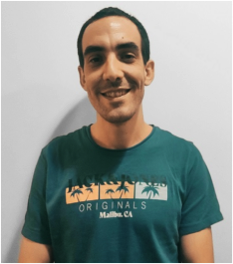
\includegraphics[width=0.30\textwidth]{david.png}
\end{wrapfigure}

\MyName{David Aleo Monteagudo}
\MySlogan{Curriculum Vitae}

\sepspace

%%% Personal details
%%% ------------------------------------------------------------
\NewPart{Datos Personales}{}

\PersonalEntry{Nacimiento}{24 de Agosto de 1986} 
\PersonalEntry{Dirección}{08290 Cerdanyola, Barcelona} 
\PersonalEntry{C.Conducir}{B}
\PersonalEntry{Teléfono}{(+34) 671 795 607}
\PersonalEntry{Mail}{\url{davidaleo@hotmail.com}}

%%% Education
%%% ------------------------------------------------------------
\NewPart{Formación}{}

\EducationEntry{CFGS Desarrollo de Aplicaciones Multiplataforma}{2018-2020}{I.E.S. LA FERRERIA}
{Desarrollo, implementación y mantenimiento de aplicaciones multiplataforma además del estudio de conceptos fundamentales de programación (estructuras de datos, algoritmos, arquitecturas)}
\sepspace

\EducationEntry{CFGS Fabricación de Productos Farmacéuticos y Afines}{2010-2011}{I.E.S. LA ROMANICA}{Gestión de las operaciones de fabricación, acondicionado y almacenamiento de productos farmacéuticos y afines.}

%%% Work experience
%%% ------------------------------------------------------------
\NewPart{Experiencia profesional}{}

\EducationEntry{DESARROLLADOR JUNIOR}{2021-present}{ATMIRA SPACE CONSULTOR S.L., Tiempo completo}{Diseño, construcción y prueba de Modelos de Procesos de Negocio (BPM) relacionados con el sector financiero, así como, colaborar en la implementación de micro servicios.}
\sepspace

\EducationEntry{DESARROLLADOR EN PRACTICAS}{2018-2020}{SIGMA UNIVERSITY MANAGEMENT, Tiempo parcial}{Aprendizaje y puesta en practica de diversas tecnologias IT, como: Javascript, Ajax, UML, JSP, Java, Html, CSS, Bootstrap.}
\sepspace

\EducationEntry{OPERARIO DE PLANTA PILOTO}{2017-2018}{LUCTA, Tiempo completo}{Síntesis de materias primas mediante operaciones de rectificación, reacción, etc. Recogida de muestras, controles y trazabilidad.}
\sepspace

\EducationEntry{OPERARIO DE FABRICACIÓN}{2015-2017}{FERRER GROUP INTERNATIONAL, Full-time}{Operario de fabricación de formas farmacéuticas sólidas. Realización de controles de calidad y procedimientos según GMP’s.}
\sepspace

\EducationEntry{OPERARIO DE FABRICACIÓN}{2014-2015}{BOEHRINGER INGELHEIM, Tiempo completo}{Operario de inspección de formas farmacéuticas líquidas acondicionadas en ampollas. Controles y trazabilidad según GMP’s.}
\sepspace

%%% Skills
%%% ------------------------------------------------------------
\NewPart{Skills}{}

\SkillsEntry{Idiomas}{Castellano (lengua materna)}
\SkillsEntry{}{Catalan (lengua materna)}
\SkillsEntry{}{Inglés (nivel B2)}


\SkillsEntry{Software - IDE's}{\textsc{NetBeans}, \textsc{Eclipse}, \textsc{IntelliJ}, \textsc{AndroidStudio}}
\SkillsEntry{}{\textsc{VisualCode}, \textsc{BPM-ibm}}
\sepspace

\SkillsEntry{Software - Frontend}{\textsc{Html}, \textsc{CSS}, \textsc{Javascript}, \textsc{Android}, \textsc{XQuery}}
\SkillsEntry{}{\textsc{Typescript}, \textsc{Bootstrap}}
\sepspace

\SkillsEntry{Software - Backend}{\textsc{Java}, \textsc{Python}, \textsc{PHP}, \textsc{SpringBoot}}
\sepspace

\SkillsEntry{Software - DataBase}{\textsc{Databases (MySQL, Oracle, Potsgre, MongoDB)}}
\sepspace

%% Objectives
%%% ------------------------------------------------------------
\NewPart{Objectivos}{}

\ObjectivesEntry{}
{Soy un desarrollador apasiado que disfruta resolviendo retos tecnológicos. Interesado en diferentes tendencias como big data, estructuras de datos, patrones de diseño. Por último pero no menos importante, me considero un miembro de equipo y formar parte de un equipo de alto rendimiento es mi objetivo.}



%%% References
%%% ------------------------------------------------------------
\NewPart{References}{}
Disponible a requerimiento
\end{document}
